\newcommand{\tab}{\hspace*{2em}}
\section{Moduł HRV1}

\subsection{Badania literaturowe}

\tab Moduł HRV1(ang. heart rate variability) służy do analizy zmiennności rytmu serca. Przeprowadza się ją,  badając różnice w  długościach interwałów RR wyznaczanych przez szczyty zespołów QRS sygnału EKG. Stosuje się do tego metody analizy statystycznej w dziedzinie czasu oraz częstotliwościowej. Dane dla tego modułu to ciąg próbek załamków R otrzymywany z modułu R\underline{  }PEAKS, natomiast szukane to parametry obu analiz oraz wykres postaci częstotliwościowej tachogramu wraz z naniesionymi zakresami obliczonych parametrów.
Problem analizy zmienności rytmu serca rozwiązuje się korzystając  z wyżej wymienionej metody analizy statystycznej (czasowej i częstotliwościowej), jednak poza zwykłym obliczaniem parametrów  korzysta się również z :

\vspace{10mm}
\begin{itemize} \itemsep0pt \parskip0pt \parsep0pt
\item modeli parametrycznych np. periodogram –wykorzystywany jako estymator w analizie widmowej,
\item modeli nieparametrycznych np. ARMA (ang. auto regressive and moving average) – regresja statystystyczna przyszłych wartości szeregu czasowego.
\end{itemize}

\vspace{10mm}

Odpowiedni dobór modelu podczas rozwiązywania problemu ma istotny wpływ na diagnozę oraz analizę złożonych parametrów fizjologicznych człowieka.

\subsection{Koncepcja omawianego rozwiązania}
\label{sec:concept}

\tab Koncepcja rozwiązania problemu odpowiedniej analizy zmienności rytmu serca jest podzielona na dwie metody, analizę statystyczną czasową oraz analizę statystyczną częstotliwościową. 

\subsubsection{Analiza statystyczna czasowa }

\tab Jest to najprostsza metoda wyliczająca szereg współczynników diagnostycznych. Za pomocą biblioteki ALGLIB, w której znajdują się odpowiednie funkcje matematyczne oraz posiądając więdzę ze statystyki matematycznej wyliczono parametry diagnostyki takie jak : 

\vspace{10mm}

\begin{itemize} \itemsep0pt \parskip0pt \parsep0pt
\item wartość średnia interwałów RR [ms],
\begin{alignat*}{3}
\overline{RR} =  \frac{1}{N}  \sum_{i=1}^{N} RR_i
\end{alignat*}
\item odchylenie standardowe interwałów RR [ms],
\begin{alignat*}{3}
SDNN =  \sqrt{\frac{1}{N-1}\sum_{i=1}^{N} (\overline{RR} - RR_i)^{2}}
\end{alignat*}
\item pierwiastek kwadratowy ze średniej kwadratów różnic pomiędzy kolejnymi dwoma interwałami RR [ms],
\begin{alignat*}{3}
RMSSD =  \sqrt{\frac{1}{N-1}\sum_{i=1}^{N-1} (RR_{i+1} - RR_i)^{2}}
\end{alignat*}
\item liczba interwałów RR, których różnica przekracza 50 [ms],
\begin{alignat*}{3}
NN50 =  \sum_{i=1}^{N-1} f_i \\
f_i =\left\{ \begin{array}{l l} 1 & \quad \text{gdy} |RR_{i+1} - RR_i|>50 \\ 0 & \quad \text{gdy}| RR_{i+1} - RR_i|\leq 50\end{array} \right.\
\end{alignat*}
\item odsetek różnic pomiędzy interwałami RR, które przekraczają 50 ms [\%],
\begin{alignat*}{3}
pNN50 =  \frac{NN50}{N-1} \times 100  \%
\end{alignat*}
\item odchylenie standardowe ze wszystkich średnich interwałów RR w 5 minutowych segmentach czasu całego zapisu [ms],
\begin{alignat*}{3}
SDANN
\end{alignat*}
\item średnia z odchyleń standardowych interwałów RR w 5 minutowych segmentach czasu całego zapisu [ms],
\begin{alignat*}{3}
SDANN  \textit{index}
\end{alignat*}
\item odchylenie standardowe różnic pomiędzy dwoma sąsiadującymi interwałami RR [ms].
\begin{alignat*}{3}
SDSD
\end{alignat*}
\end{itemize}
gdzie:
\begin{itemize}
\item $N$ - ilość próbek tachogramu
\item $RR_i$ - wartość i-tego interwału $RR$
\end{itemize}

\vspace{10mm}

\subsubsection{Analiza statystyczna częstotliwościowa }


\tab Jest to bardziej złożona metoda analizy parametrów zmienności rytmu serca, operająca się o dyskretną transformatę Fouriera, rzadziej funkcję autokorelacji. Do jej zastosowania użyto biblioteki ALGLIB. Przed zastosowaniem samej transformaty Fouriera skorzystano z krzywej splajn odnośnie danych wejściowych. Dzięki takim operacją obliczono następujące parametry analizy częstotliwościowej:

\vspace{10mm}

\begin{itemize} \itemsep0pt \parskip0pt \parsep0pt
\item całkowita moc widma ($\leq$ 0.4 Hz) $[ms^{2}]$,
\begin{alignat*}{3}
TP
\end{alignat*}
\item moc widma w zakresie wysokich częstotliwości (0.15 - 0.4 Hz) $[ms^{2}]$ ,
\begin{alignat*}{3}
HF
\end{alignat*}
\item moc widma w zakresie niskich częstotliwości (0.04 - 0.15 Hz) $[ms^{2}]$,
\begin{alignat*}{3}
LF
\end{alignat*}
\item moc widma w zakresie bardzo niskich częstotliwości (0.003 - 0.04 Hz) $[ms^{2}]$,
\begin{alignat*}{3}
VLF
\end{alignat*}
\item moc widma w zakresie ultra niskich częstotliwości ($\leq$ 0.003 Hz) $[ms^{2}]$,
\begin{alignat*}{3}
ULF
\end{alignat*}
\item stosunek mocy widm w zakresie niskich częstotliwości do wysokich częstotliwości.
\begin{alignat*}{3}
LFHF = \frac{LF}{HF}
\end{alignat*}
\end{itemize}

\vspace{10mm}

Po dokonaniu wyliczeń wszystkich parametrów analizy częstotliwościowej ustawiono dane potrzebne
do narysowania wykresu widma mocy sygnału EKG z odpowiednimi przedziałami mocy. Przykłady takich wykresów są umieszczone
w sekcji \ref{sec:rezultat}.

\subsection{Realizacja i wnioski}
\label{sec:rezultat}

\tab Po zaprogramowaniu wszystkich koniecznych funkcji wyliczających odpowiednie parametry czasowe i częstotliwościowe oraz funkcji odpowiedzialnych za rysowanie wykresów widma mocy sygnału EKG przystąpiono do przetestowania działania modułu na 5 różnych  danych wejściowych. W tabeli \ref{tab:stats} widoczne są wszystkie wyliczone parametry analizy statystycznej dla 5 różnych sygnałów EKG.

\vspace{5mm}

\begin{table}[ht]
\caption{Analiza statystyczna}
\label{tab:stats}
\begin{tabular}{|c|c|c|c|c|c|}
 \hline
 & 1 & 2 & 3 & 4 & 5\\
\hline
Mean[ms] & 794.15  & 865.42 & 932.61 & 811.53 & 752.76\\
SDNN[ms] & 48.89 & 48.70 & 331.29 & 135.28 & 192.25\\
RMSSD[ms] & 63.36 & 35.72 & 497.84 & 135.56 & 282.50\\
RR50 & 219.00 & 211.00 & 1266.00 & 534.00 & 335.00\\
RR50 Ratio[\%] & 9.64 & 10.13 & 65.49 & 24.03 & 13.98\\
SDANN[ms] & 33.05 & 20.74 & 72.86 & 14.80 & 19.38\\
SDANN Index[ms] & 42.83 & 42.27 & 307.49 & 117.46 & 122.20\\
SDSD[ms] & 54.69 & 24.01 & 377.84 & 118.57 & 273.63\\
\hline
\end{tabular}
\end{table}

\vspace{5mm}

Jak widać z tabeli \ref{tab:stats} parametry dla pomiaru 1 oraz 2 zgadzają się z typowymi wartościami dla sygnału EKG przeprowadzonego na zdrowym pacjencie. Pozostałem pomiary a szczególnie pomiar 3 oraz 5 posiadają wartości znacząco odbiegające od odpowiednich, co może świadczyć o tym, że pacjent posiada zaburzenia pracy serca.
Dla porównania na rysunku \ref{fig:big} przedstawiono parę parametrów analizy czasowej zmienności rytmu serca u zdrowego człowieka w wieku od 40 do 69 lat wg. Biggera

\vspace{5mm}

\begin{figure}[ht]
\centering
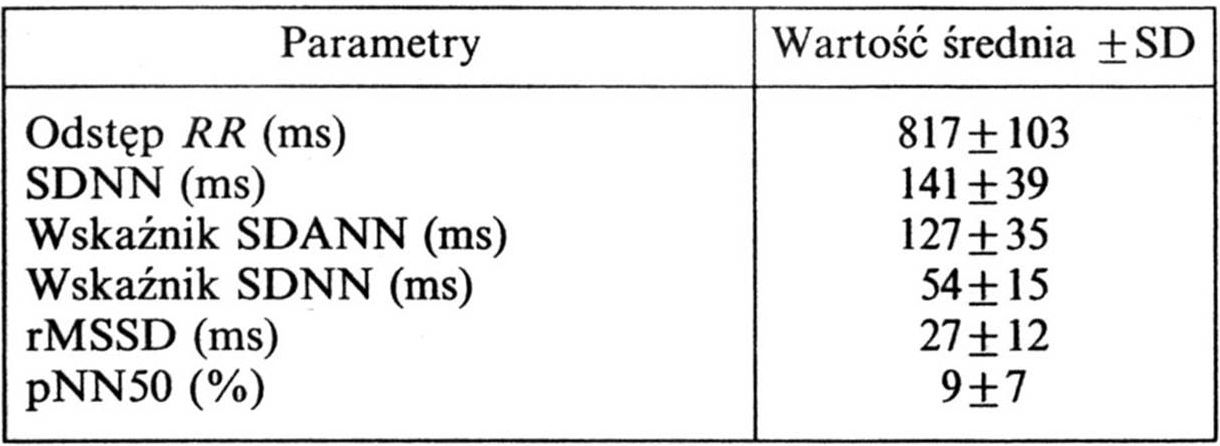
\includegraphics[scale=0.4]{HRV1/foty/bigger.jpg}
\caption{Analiza czasowa wg. Biggera}
\label{fig:big}
\end{figure}
\newpage
Powyższe rozważania dotyczą jedynie charakterystyki czasowej statycznej, natomiast dużo więcej można się dowiedzieć przeprowadzając charakterystykę częstotliwościową. W tabeli \ref{tab:freq} umieszczone są wyliczone parametry analizy częstotliwościowej dla takich samych sygnałów jak w przypadku analizy statycznej.



\begin{table}[ht]
\caption{Analiza częstotliwościowa}
\label{tab:freq}
\begin{tabular}{|c|c|c|c|c|c|}
 \hline
 & 1 & 2 & 3 & 4 & 5\\
\hline
TP[$ms^{2}$] & 3190.00 & 4132.00 & 208550.00 & 17268.00 & 238756.00\\
HF[$ms^{2}$] & 1846.00 & 1384.00 & 83800.00 & 8581.00 & 11153.00\\
LF[$ms^{2}$] & 179.00 & 478.00 & 38673.00 & 4440.00 & 127614.00\\
VLF[$ms^{2}$] & 627.00 & 1750.00 & 73051.00 & 3209.00 & 87569.00\\
ULF[$ms^{2}$] & 536.00 & 519.00 & 13024.00 & 1036.00 & 12419.00\\
LFHF[\%] & 9.73 & 34.56 & 46.15 & 51.75 & 1144.17\\
\hline
\end{tabular}
\end{table}



Oceniając wartości poszczególnych parametrów analizy częstotliwościowej widoczne w tabeli \ref{tab:freq} dochodzi się do podobnego wniosku jak w przypadku analizy czasowej. Wartości w pomiarach 3, 4 oraz 5 odbiegają od parametrów zmienności rytmu serca u zdrowych dorosłych osób.

\tab Kolejnym krokiem w analizie częstotliwościowej jest narysowanie wykresu mocy widma wyrażonego w milisekundach do kwadratu w stosunku do częstotliwości odpowiedniego zakresu widma. Jak zostało opisane w sekcji \ref{sec:concept} najpierw skorzystano z krzywej splajn odnośnie danych wejściowych co obrazuje rysunek \ref{fig:rr1}. Jest to wykres RR dla pierwszego sygnału EKG użytego podczas wyliczania parametrów czasowych oraz częstotliwościowych.

\vspace{5mm}

\begin{figure}[ht]
\centering
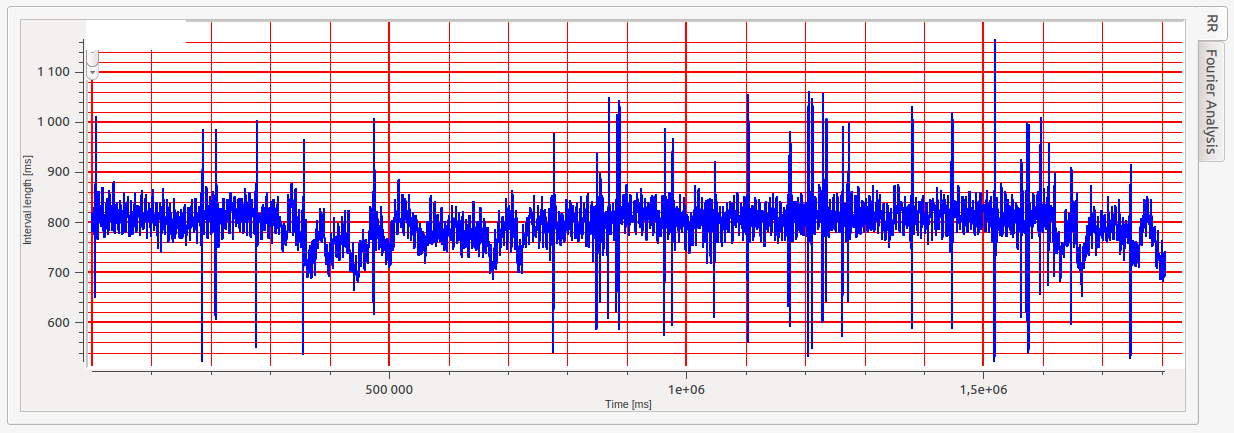
\includegraphics[scale=0.4]{HRV1/foty/100/RR1.png}
\caption{Wykres RR dla pierwszego pomiaru}
\label{fig:rr1}
\end{figure}

\vspace{5mm}

\newpage

Następnie można  przeprowadzić szybką transformatę Fouriera, która jeżeli wykres RR był w miarę okresowy powinna dać jeden wyróżniający się pik w środkowej części wykresu gęstości mocy widma. Na rysunkach \ref{fig:four1}, \ref{fig:four2}, \ref{fig:four3}, \ref{fig:four4}, \ref{fig:four5} widoczne są kolejno przeprowadzone transformaty Fouriera na sygnałach EKG kolejnych 5 pomiarów. Cały czas korzystano z tych samych pomiarów co przy wyliczaniu parametrów czasowych i częstotliwościowych.

\vspace{5mm}

\begin{figure}[ht]
\centering
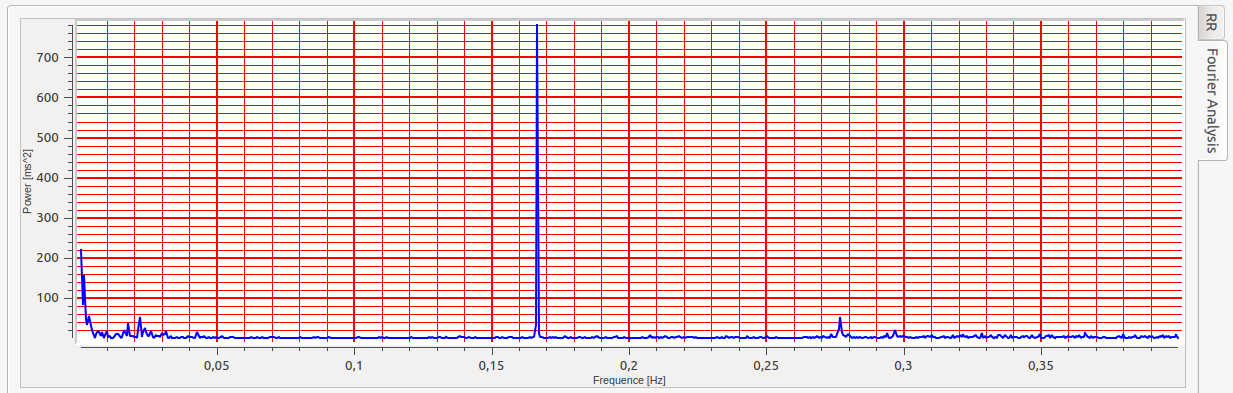
\includegraphics[scale=0.4]{HRV1/foty/100/fourier1.png}
\caption{Wykres transformaty Fouriera dla pierwszego pomiaru}
\label{fig:four1}
\end{figure}

\vspace{5mm}

\begin{figure}[ht]
\centering
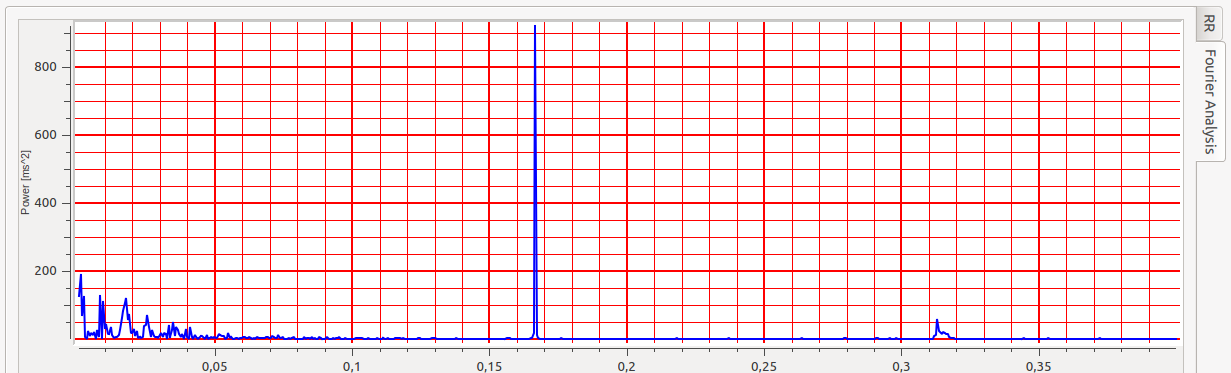
\includegraphics[scale=0.35]{HRV1/foty/103/fourier2.png}
\caption{Wykres transformaty Fouriera dla drugiego pomiaru}
\label{fig:four2}
\end{figure}



\begin{figure}[ht]
\centering
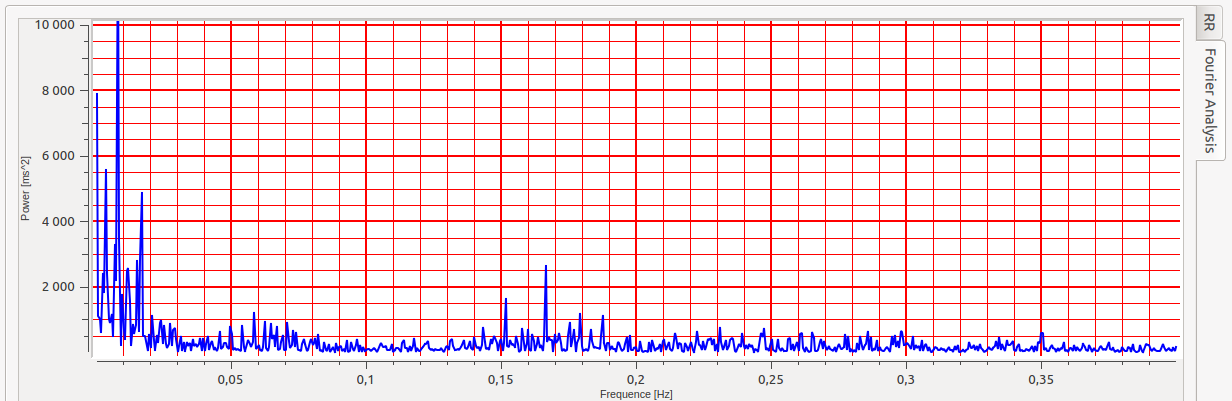
\includegraphics[scale=0.35]{HRV1/foty/106/fourier3.png}
\caption{Wykres transformaty Fouriera dla trzeciego pomiaru}
\label{fig:four3}
\end{figure}

\vspace{5mm}

\begin{figure}[H]
\centering
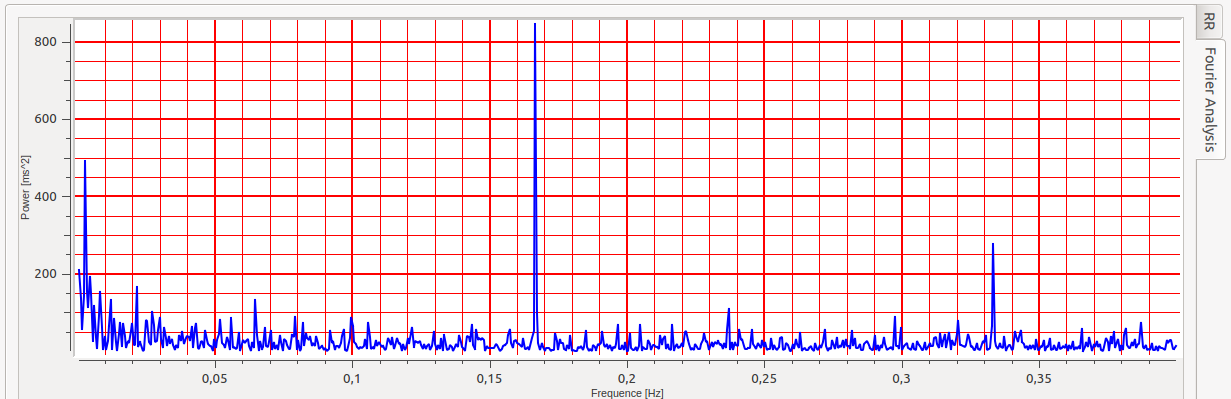
\includegraphics[scale=0.35]{HRV1/foty/111/fourier4.png}
\caption{Wykres transformaty Fouriera dla czwartego pomiaru}
\label{fig:four4}
\end{figure}

\vspace{5mm}

\begin{figure}[H]
\centering
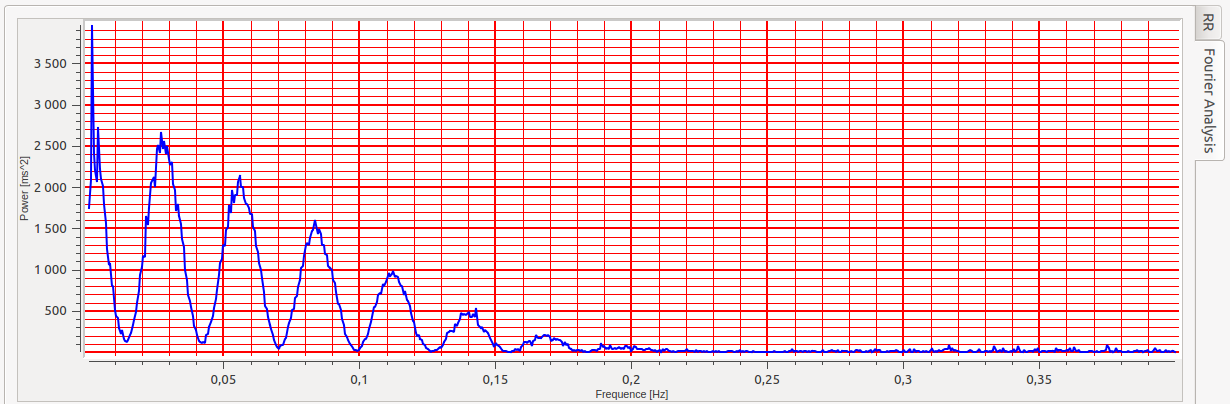
\includegraphics[scale=0.35]{HRV1/foty/116/fourier5.png}
\caption{Wykres transformaty Fouriera dla piątego pomiaru}
\label{fig:four5}
\end{figure}





Po obejrzeniu wykresów transformaty Fouriera dla 5 różnych sygnałów EKG można dojść do wniosku, że najlepszy wynik, a co za tym idzie najlepsza praca serca występuje dla pacjentów z sygnałem EKG pierwszym oraz drugim. Są one najbardziej zbliżone do normalnej pracy serca zdrowego dorosłego człowieka. Gorsze wyniki uzyskujemy przy sygnale czwartym, natomiast pomiar trzeci oraz piąty świadczą o tym, że dane wejściowe dotyczyły człowieka z prawdopodobnymi zaburzeniami serca. Wykresy Fouriera w tych obu przypadkach nie pokazują jednoznacznej częstotliwości oraz wartość mocy widma jest zdecydowanie za duża w obu przypadkach.\\
\tab Moduł HRV1 według oceny autorów został poprawnie zinterpretowany i zaprogramowany. Świadczą o tym wyniki parametrów obu analiz oraz wykresy częstotliwościowe. Porównując wyniki modułu z przykładowymi wynikami zaczerpniętymi z internetu można znaleźć duże podobieństwo, szczególnie dla sygnałów EKG zdrowego, dorosłego człowieka. \\
W ostatniej sekcji \ref{sec:diag} został przedstawiony diagram klas oraz sekwencj programu zaprogramowanego na potrzeby modułu HRV1.


\subsection{Diagramy klas i sekwencji}
\label{sec:diag}

\subsubsection{Diagram klas}

\begin {tikzpicture}

	\begin{class}[text width = 13cm]{HRV1MainModule}{0,0}
		\attribute{- dividedPeaks : QVector<QVector<double>*>}
		\attribute{- peaks : QVector<double>}
		\attribute{- RRDifferences : QVector<double>}
		\attribute{- samplingFrequency : double}
		\attribute{- toReturnStatistical : HRV1BundleStatistical}
		\attribute{- splineInterpolant : spline1dinterpolant}
		\attribute{- fftArray : complex\_1d\_array}
		\attribute{- toReturnFrequency : HRV1BundleFrequency}

		\operation{+ prepare(RRPeaks : QVector<int>*, samplingFrequency : int = 1000)}
		\operation{+ evaluateStatistical() : HRV1BundleStatistical}
		\operation{+ evaluateFrequency() : HRV1BundleFrequency}
		\operation{- evaluateRRMeanEntirety()}
		\operation{- evaluateSDNNEntirety()}
		\operation{- evaluateRMSSD()}		
		\operation{- evaluateNN50()}
		\operation{- evaluatepNN50()}
		\operation{- evaluateSDANN()}
		\operation{- evaluateSDANNindex()}
		\operation{- evaluateSDSD()}
		\operation{- evaluateSplainInterpolation()}
		\operation{- evaluateFFT()}
		\operation{- evaluateTP()}
		\operation{- evaluateHF()}
		\operation{- evaluateLF()}
		\operation{- evaluateVLF()}
		\operation{- evaluateULF()}
		\operation{- evaluateLFHF()}

	\end{class}

	\begin{class}{HRV1BundleStatistical}{-5.0, -15.0}
		\attribute{RRMean : double}
		\attribute{SDNN : double}
		\attribute{RMSSD : double}
		\attribute{NN50 : double}
		\attribute{pNN50 : double}
		\attribute{SDANN : double}
		\attribute{SDANNindex : double}
		\attribute{SDSD : double}
	

	\end{class}

	\begin{class}{HRV1BundleFrequency}{5.0, -15.0}
		\attribute{xData : QVector<double>*}
		\attribute{yData : QVector<double>*}
		\attribute{rrXData : QVector<double>*}
		\attribute{rrYData : QVector<double>*}
		\attribute{TP : double}
		\attribute{HF : double}
		\attribute{LF : double}
		\attribute{VLF : double}
		\attribute{ULF : double}
		\attribute{LFHF : double}

	\end{class}

	\aggregation{ HRV1MainModule}{output}{1}{HRV1BundleStatistical}
	\aggregation{ HRV1MainModule}{output}{1}{HRV1BundleFrequency}

\end{tikzpicture}

\subsubsection{Diagram sekwencji}

\begin{sequencediagram}
	\newthread{t}{ : Controller}
	\newinst[2]{i}{ : HRV1MainModule}

	\begin{messcall}{t}{prepare()}{i}
	\end{messcall}

	\begin{call}{t}{evaluateStatistical()}{i}{toReturnStatistical}
		\begin{callself}{i}{evaluateRRMeanEntirety()}{}
		\end{callself}
		\begin{callself}{i}{evaluateSDNNEntirety()}{}
		\end{callself}
		\begin{callself}{i}{evaluateRMSSD()}{}
		\end{callself}
		\begin{callself}{i}{evaluateNN50()}{}
		\end{callself}
		\begin{callself}{i}{evaluatepNN50()}{}
		\end{callself}
		\begin{callself}{i}{evaluateSDANN()}{}
		\end{callself}
		\begin{callself}{i}{evaluateSDANNindex()}{}
		\end{callself}
		\begin{callself}{i}{evaluateSDSD()}{}
		\end{callself}
	\end{call}
\end{sequencediagram}
\begin{sequencediagram}
	\newthread{t}{ : Controller}
	\newinst[2]{i}{ : HRV1MainModule}

	\begin{call}{t}{evaluateFrequency()}{i}{toReturnFrequency}
		\begin{callself}{i}{evaluateSplainInterpolation()}{}
		\end{callself}
		\begin{callself}{i}{evaluateFFT()}{}
		\end{callself}
		\begin{callself}{i}{evaluateTP()}{}
		\end{callself}
		\begin{callself}{i}{evaluateHF()}{}
		\end{callself}
		\begin{callself}{i}{evaluateLF()}{}
		\end{callself}
		\begin{callself}{i}{evaluateVLF()}{}
		\end{callself}
		\begin{callself}{i}{evaluateULF()}{}
		\end{callself}
		\begin{callself}{i}{evaluateLFHF()}{}
		\end{callself}
	\end{call}

\end{sequencediagram}